\documentclass[a4paper,10pt]{article}
\usepackage[utf8]{inputenc}
\usepackage{graphicx}
\graphicspath{ {./code/} }

\title{\textbf{Behavior of different agents} \\ 
\textbf{Project}}

\author{Emil Ståhl and Peyman Peirovifar}

\begin{document}

\maketitle

\section{Introduction}
This report covers an experiment that demonstrates and analyzes the behaviors and interactions between different types of 
agents by simulating a festival event. The agents have their own personal characteristics, preferences and intentions of 
visiting the festival. The experiment is set to investigate what happens when these agents meet and interact with each other. How will the agents change each others behaviors?
The experiment is conducted as a simulation using the GAMA platform which is an open-source environment for spatially 
explicit multiagent simulations. 


\maketitle
\section{Approach}
This sections describes the method and approach used during the project work. 

\maketitle
\subsection{Simulation}
To simulate the festival we used some parts from our previous work such as ”GAMA and Agents”, ”Negotiation and Communication 
(FIPA)” and ”Coordination and Utility”. As an example, the dance floors from the third project is reused in this experiment. 
Similar to the first work in ”GAMA and Agents” there are places for the agents to visit when desired. These places are dance 
floor, store,  and pubs. Furthermore, each agent has a predetermined personality trait which determines how they will 
interact with other agents, accept proposals and move around the festival area. 
The simulation has the following structure.

\begin{itemize}
    \item 5 types of agents totaling a number of 50 
    \item Rules of how the agents interact with other agents
    \item Each guest has 3 personal traits of a varying intensity
    \item Three types of places where the agents can meet
    \item Continuously running simulation
    \item FIPA protocol for long distance messaging
\end{itemize}

\clearpage
\maketitle

\section{Experiment}
This section describes the implementation of the simulation.

\maketitle
\subsection{Locations}
The simulation is created with three types of locations where the festival guests can meet and interact. These places are:

\begin{itemize}
    \item Pub
    \item DanceFloor
    \item Store
    
\end{itemize}

The simulation is by default set to have 9 of these places but can easily be changed by altering the number\_of\_places variable. 

\subsection{Guests}
A species called ”Guest” is created to handle the logic of the agents moving around and interacting with each other. The number of guests in the simulation is by default set to 50 and can be changed by altering the number\_of\_guests” variable. 

\subsubsection{Personality traits}
Every guest presented in the simulation are given three types of personality traits with a value [0, 10] that determines how strong each personality trait are. The value is randomly initialized once the simulation is started. The different types of traits are:

\begin{itemize}
    \item Kindness
    \item Sympathetic
    \item Charitable
    
\end{itemize}
The degree of each personality trait determines how the guest will interact with other guests and to what extent they accept or reject potential proposals from other guests. Furthermore, this acceptance rate of each guest is accumulated in a global counter and presented in the form of a pie chart in order to monitor how it changes during the simulation. 

\subsubsection{Attributes}
In addition to the guests personality traits, each guest is also given one of five personality attributes that decides how the guest will interact with other types of guests with other attributes as well as where the guest prefer to hangout within the festival area. The attributes are:

\begin{itemize}
    \item Extrovert
    \item Introvert
    \item Juicehead
    \item Journalist
    \item Salesman
\end{itemize}

The preference of each guest is displayed in the table below:

\begin{center}
\begin{tabular}{ |c|c| } 
 \hline
 \textbf{Attribute} & \textbf{Preffered Place} \\

 Extrovert & DanceFloor \\ 
 Introvert & Store  \\ 
 Juicehead & Pub  \\
 Journalist & None \\
 Salesman & None \\
 
 \hline
\end{tabular}
\end{center}

\subsection{Interactions and proposals}

The goal of this experiment is to investigate what happens when different types of agents meet and interact with each other. These interactions are in the form of making proposals to other agents regarding if they are interested in, for example, join them for a drink. These proposals can be made either on the way towards a place or at the place itself. However, the guest needs to be within at least 5 meters from another guest in order to initiate the proposal. 

\subsubsection{Time limit for proposals}
In order to avoid that a guest makes multiple proposals to the same counterpart over and over again an attribute is given to each guest. This attribute will be reset every 200 - 400 simulation cycles and when that happens the guest will be given a new target point to move to. This prohibits guests from being stuck and ensures a smooth running simulation. 

\subsection{Agents and rules}
Every guest is given a set of rules that determine how they will interact with other agents and if they will accept proposals from others. The rules is in the form of a floating point between [0,1] that is predetermined at creation. The rules are defined as an attribute:

\begin{center}
\begin{tabular}{ |c| } 
 \hline
 \textbf{Agent Rules} \\
 Extrovert\_attribute \\
 Introvert\_attribute \\
 Juicehead\_attribute \\
 Journalist\_attribute \\
 Salesman\_attribute \\
 \hline
\end{tabular}
\end{center}

A proposal from one agent to another is determined by the corresponding value of the guest making the proposal. For example, if a guest receives a proposal from a guest with the type of a introvert and the receiving guest has an attribute rule of 1.0 as Introvert\_attribute the proposal will always be accepted. Similarly, an attribute of 0.0 will result in that the proposal being rejected at all times.

\subsubsection{Priority of personality traits and agent rules}
The personality traits given to each agent has absolute priority over the agent rules. If a personality trait is \textless 5.0 the proposal from another agent will always be rejected regardless if the agent has a high attribute for interacting with that type of agent. 

\subsection{Implementing spread of infection}
During the time this project was conducted the world is currently going thru the COVID-19 pandemic. Therefore we think it’s interesting to see how a virus like this can spread around a festival and infect the guests while they interact with each other.
The five personality traits are now added to a group of other agents that have the same personality as themselves. The groups are challenging each other for which team that will be left when all other teams have been infected with the virus. To manage this, the simulation is extended with an instructor agent that handles this spread of disease. The instructor will at the start of the simulation infect one team member of each team with the virus. The guests are then free to wander around the festival and interact with each other according to the rules explained in previous chapters. However, when an agent accepts a proposal for interacting from another infected agent, the accepting agent will be infected as well and carry on the virus to other guests it interacts with.  

\subsubsection{Communication thru FIPA}
The instructor species are responsible for keeping track of what’s happening during the festival in regards to this spread of infection competition. This communication is done in real time thru the communication protocol FIPA. The instructor will when all members of a time has been infected remove this team from the competition. In addition to this, the instructor is also updating a leader board that shows the state of each team. 


\section{Results}

This section shows the results from running the experiment

\subsection{Acceptance and rejection rate}

The goal if this experiment is to measure the acceptance and rejection rate of the proposals made between all the agents. This is done by accumulating the global counters acceptance\_count and rejection\_count. These variables are updated in the if-clauses of the interact reflex. 

\begin{verbatim}

    if self.kindness>=5 {
		decider <- flip(self.Extrovert_attribute);
		if decider=true {
			acceptance_count <- acceptance_count + 1;
        }
    }
    
    else if self.kindness<5 {
	    decider <- false;
	    rejection_count <- rejection_count + 1;
    }
\end{verbatim}

In the experiment a chart is displayed with these values and is continuously updated throughout the entirety of the simulation. The results are shown in the chart below:

\begin{center}{}
\centering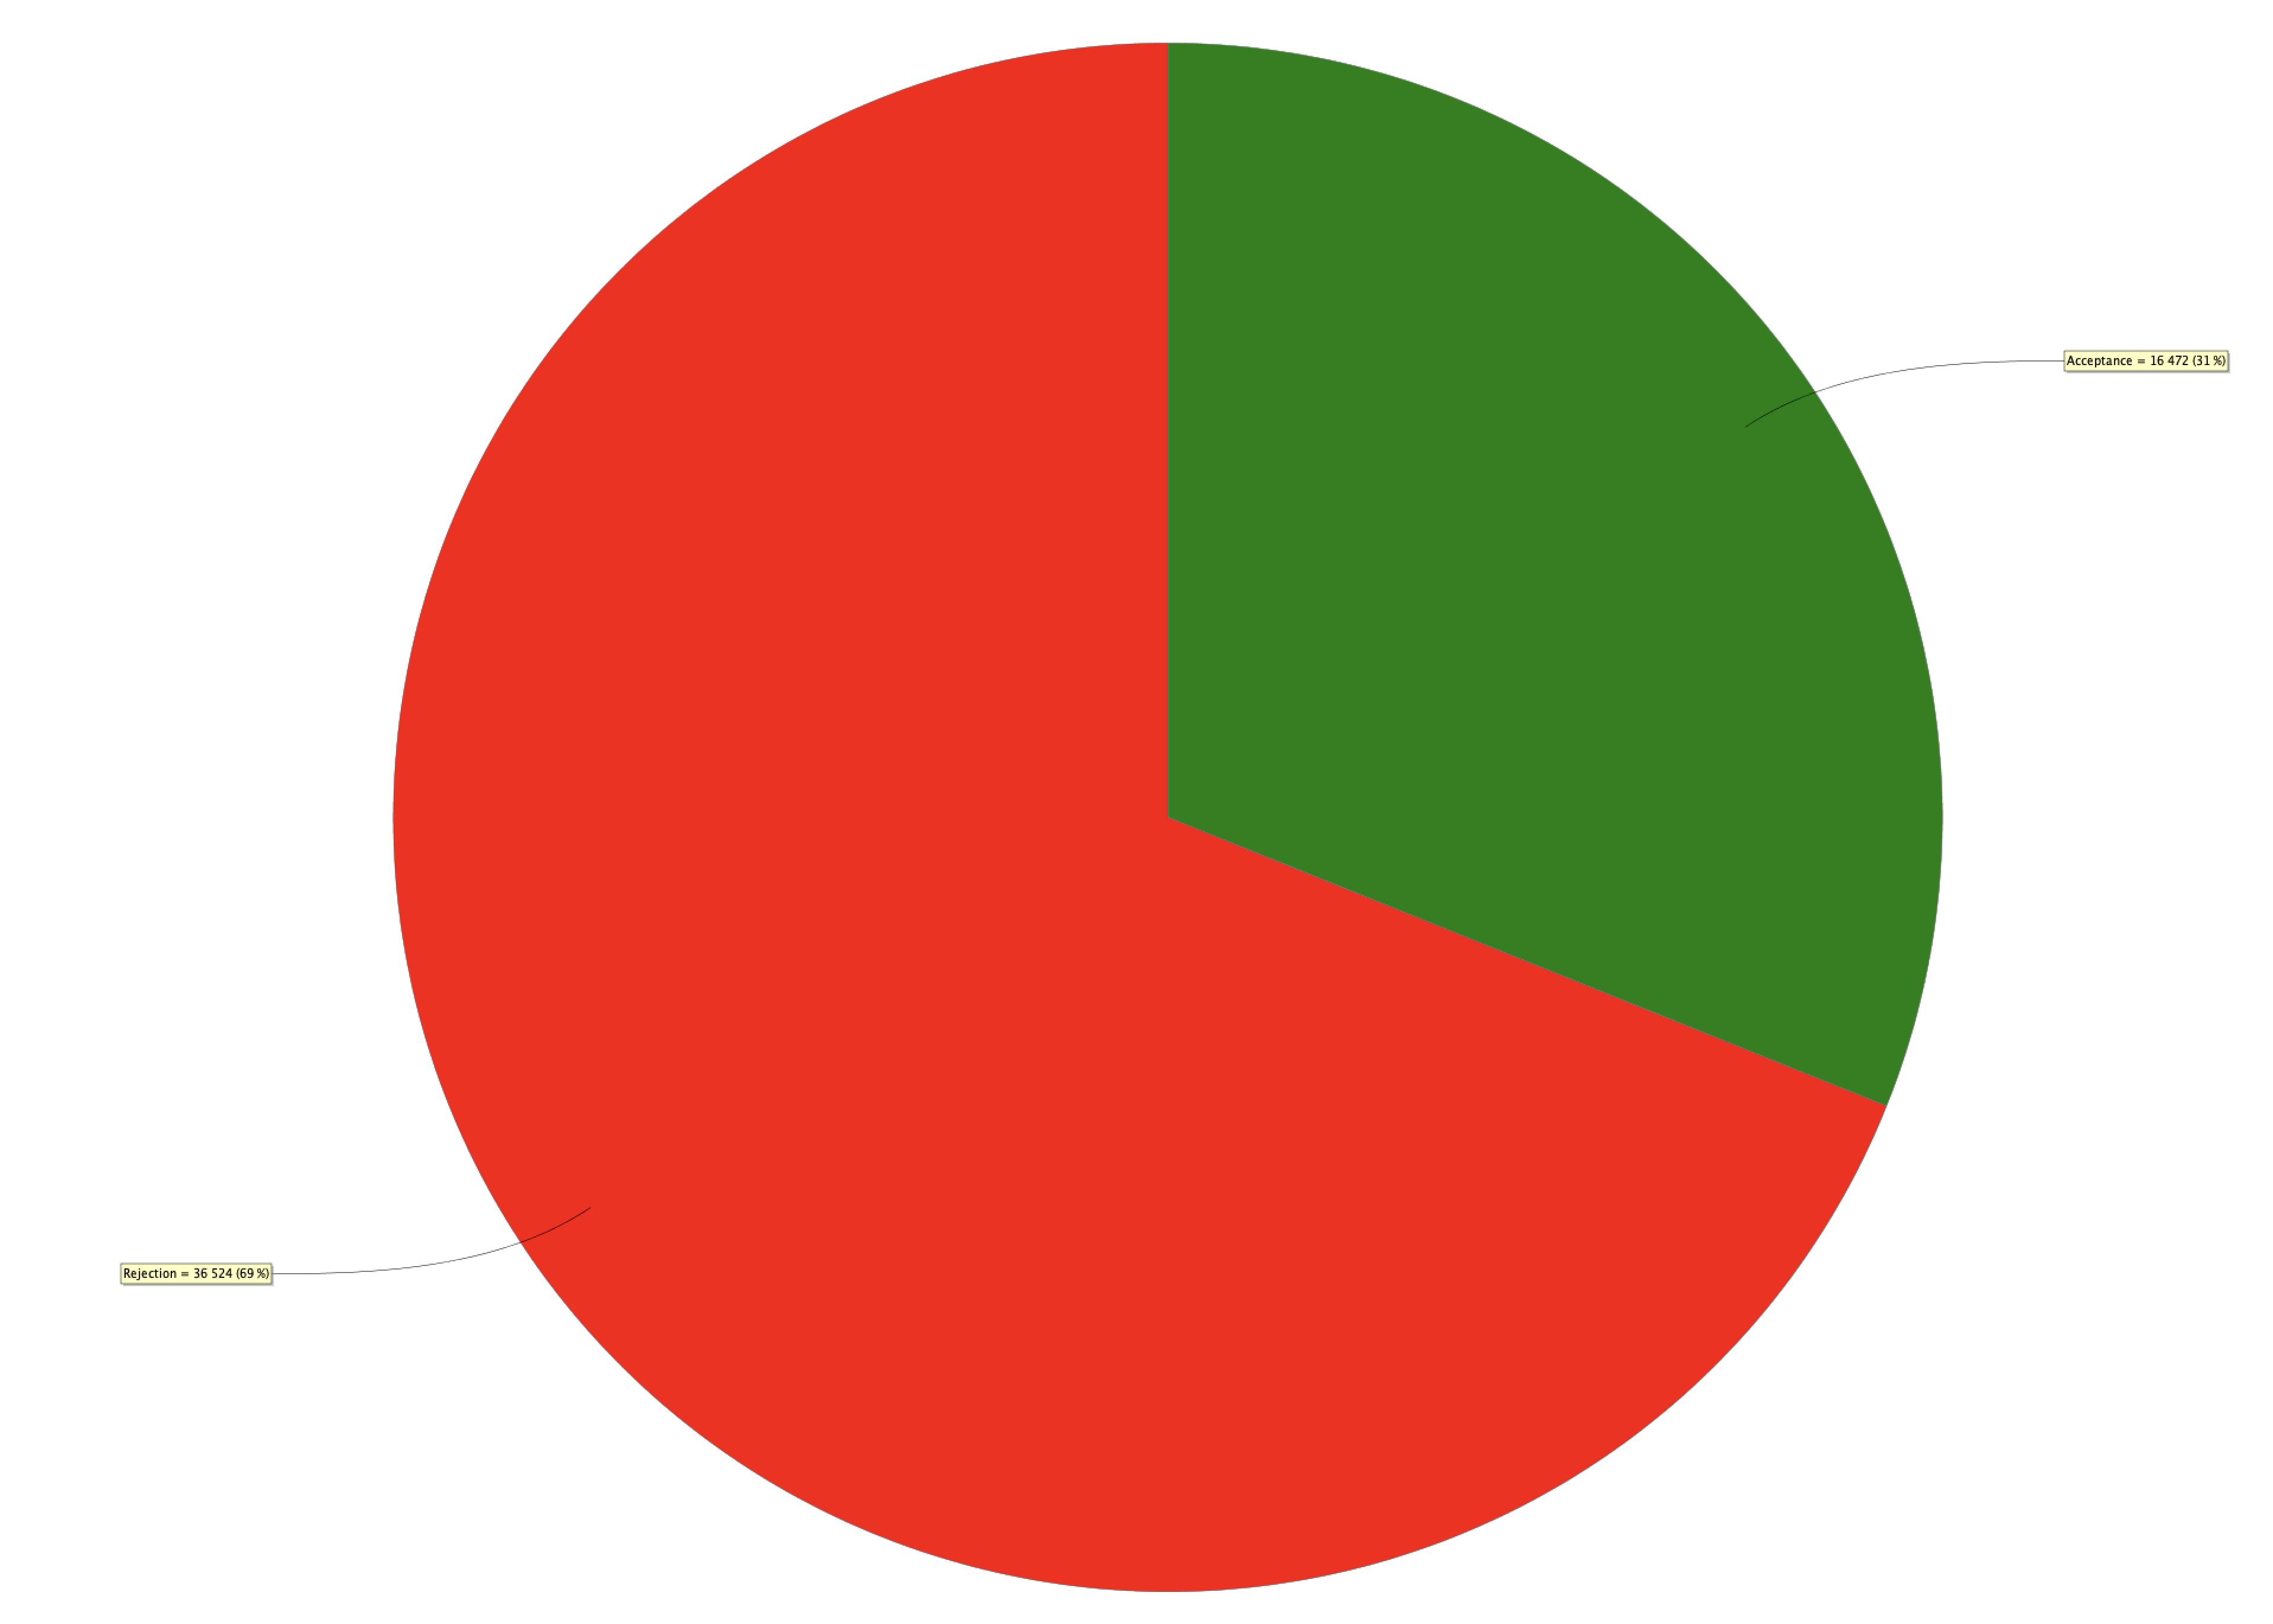
\includegraphics[scale=0.05]{original_exp.png}\par
\end{center}

As seen in the chart the rejection rate is \textasciitilde 69\% and the acceptance rate \textasciitilde 31\%. Interestingly, this distribution is the same every instance of the simulation. This is most likely due to the way the agent rule attributes and personality traits are implemented, the simulation will therefore by probabilistic distribution always converge to these values shown in the chart above. 

\subsection{Altering the rules}
This sections shows the results of altering the original rules described in the previous sections. Every alteration is compared to the original set of rules.

\subsubsection{Lowering threshold level}
In the following chart, the threshold level for the personality traits was lowered from 5.0 to 3.0. The acceptance rate, self-evidently, increases to \textasciitilde 68\%.

\begin{center}{}
\centering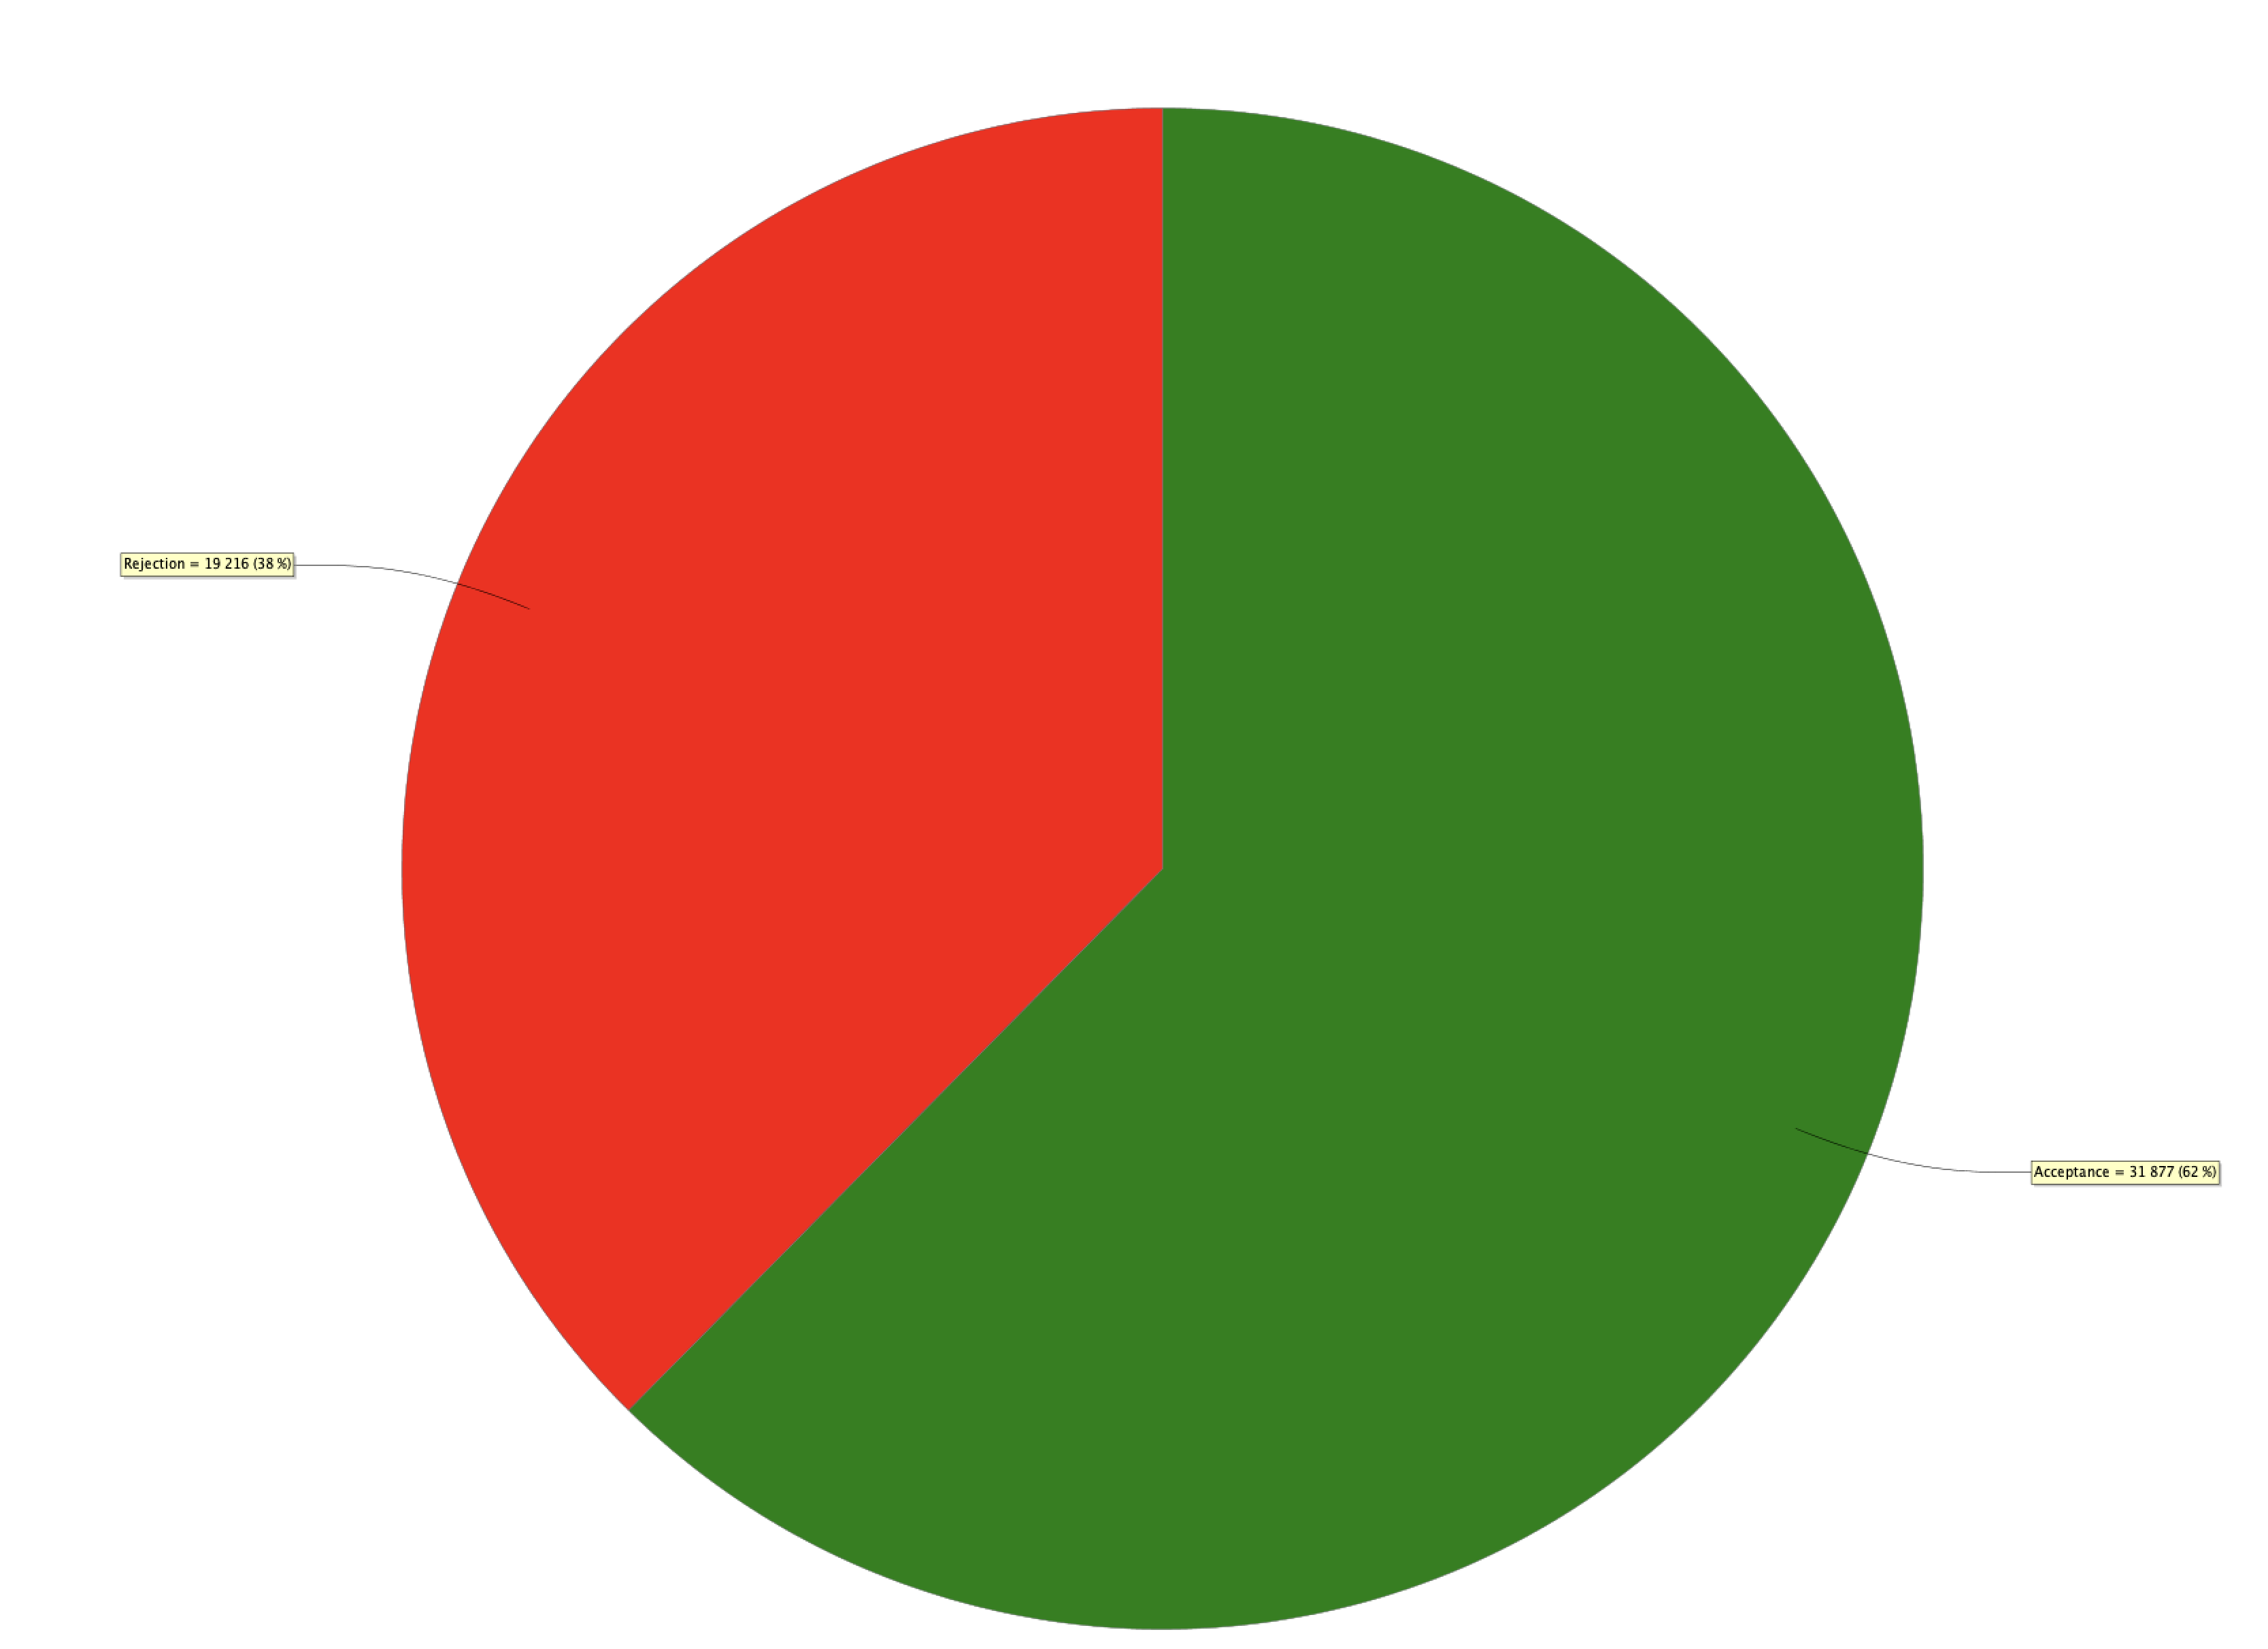
\includegraphics[scale=0.05]{lowerthreshold.png}\par
\end{center}

\subsubsection{Removing the time limit}
By removing the time limit attribute of each agent that prohibits them from making multiple proposals to the same agent it can be seen that the acceptance level drops significantly. This is because agents are now making new proposals to the same agent even after they have been rejected, which deteriorates their ability to move around and meet new agents that better match their preferences.

\begin{center}{}
\centering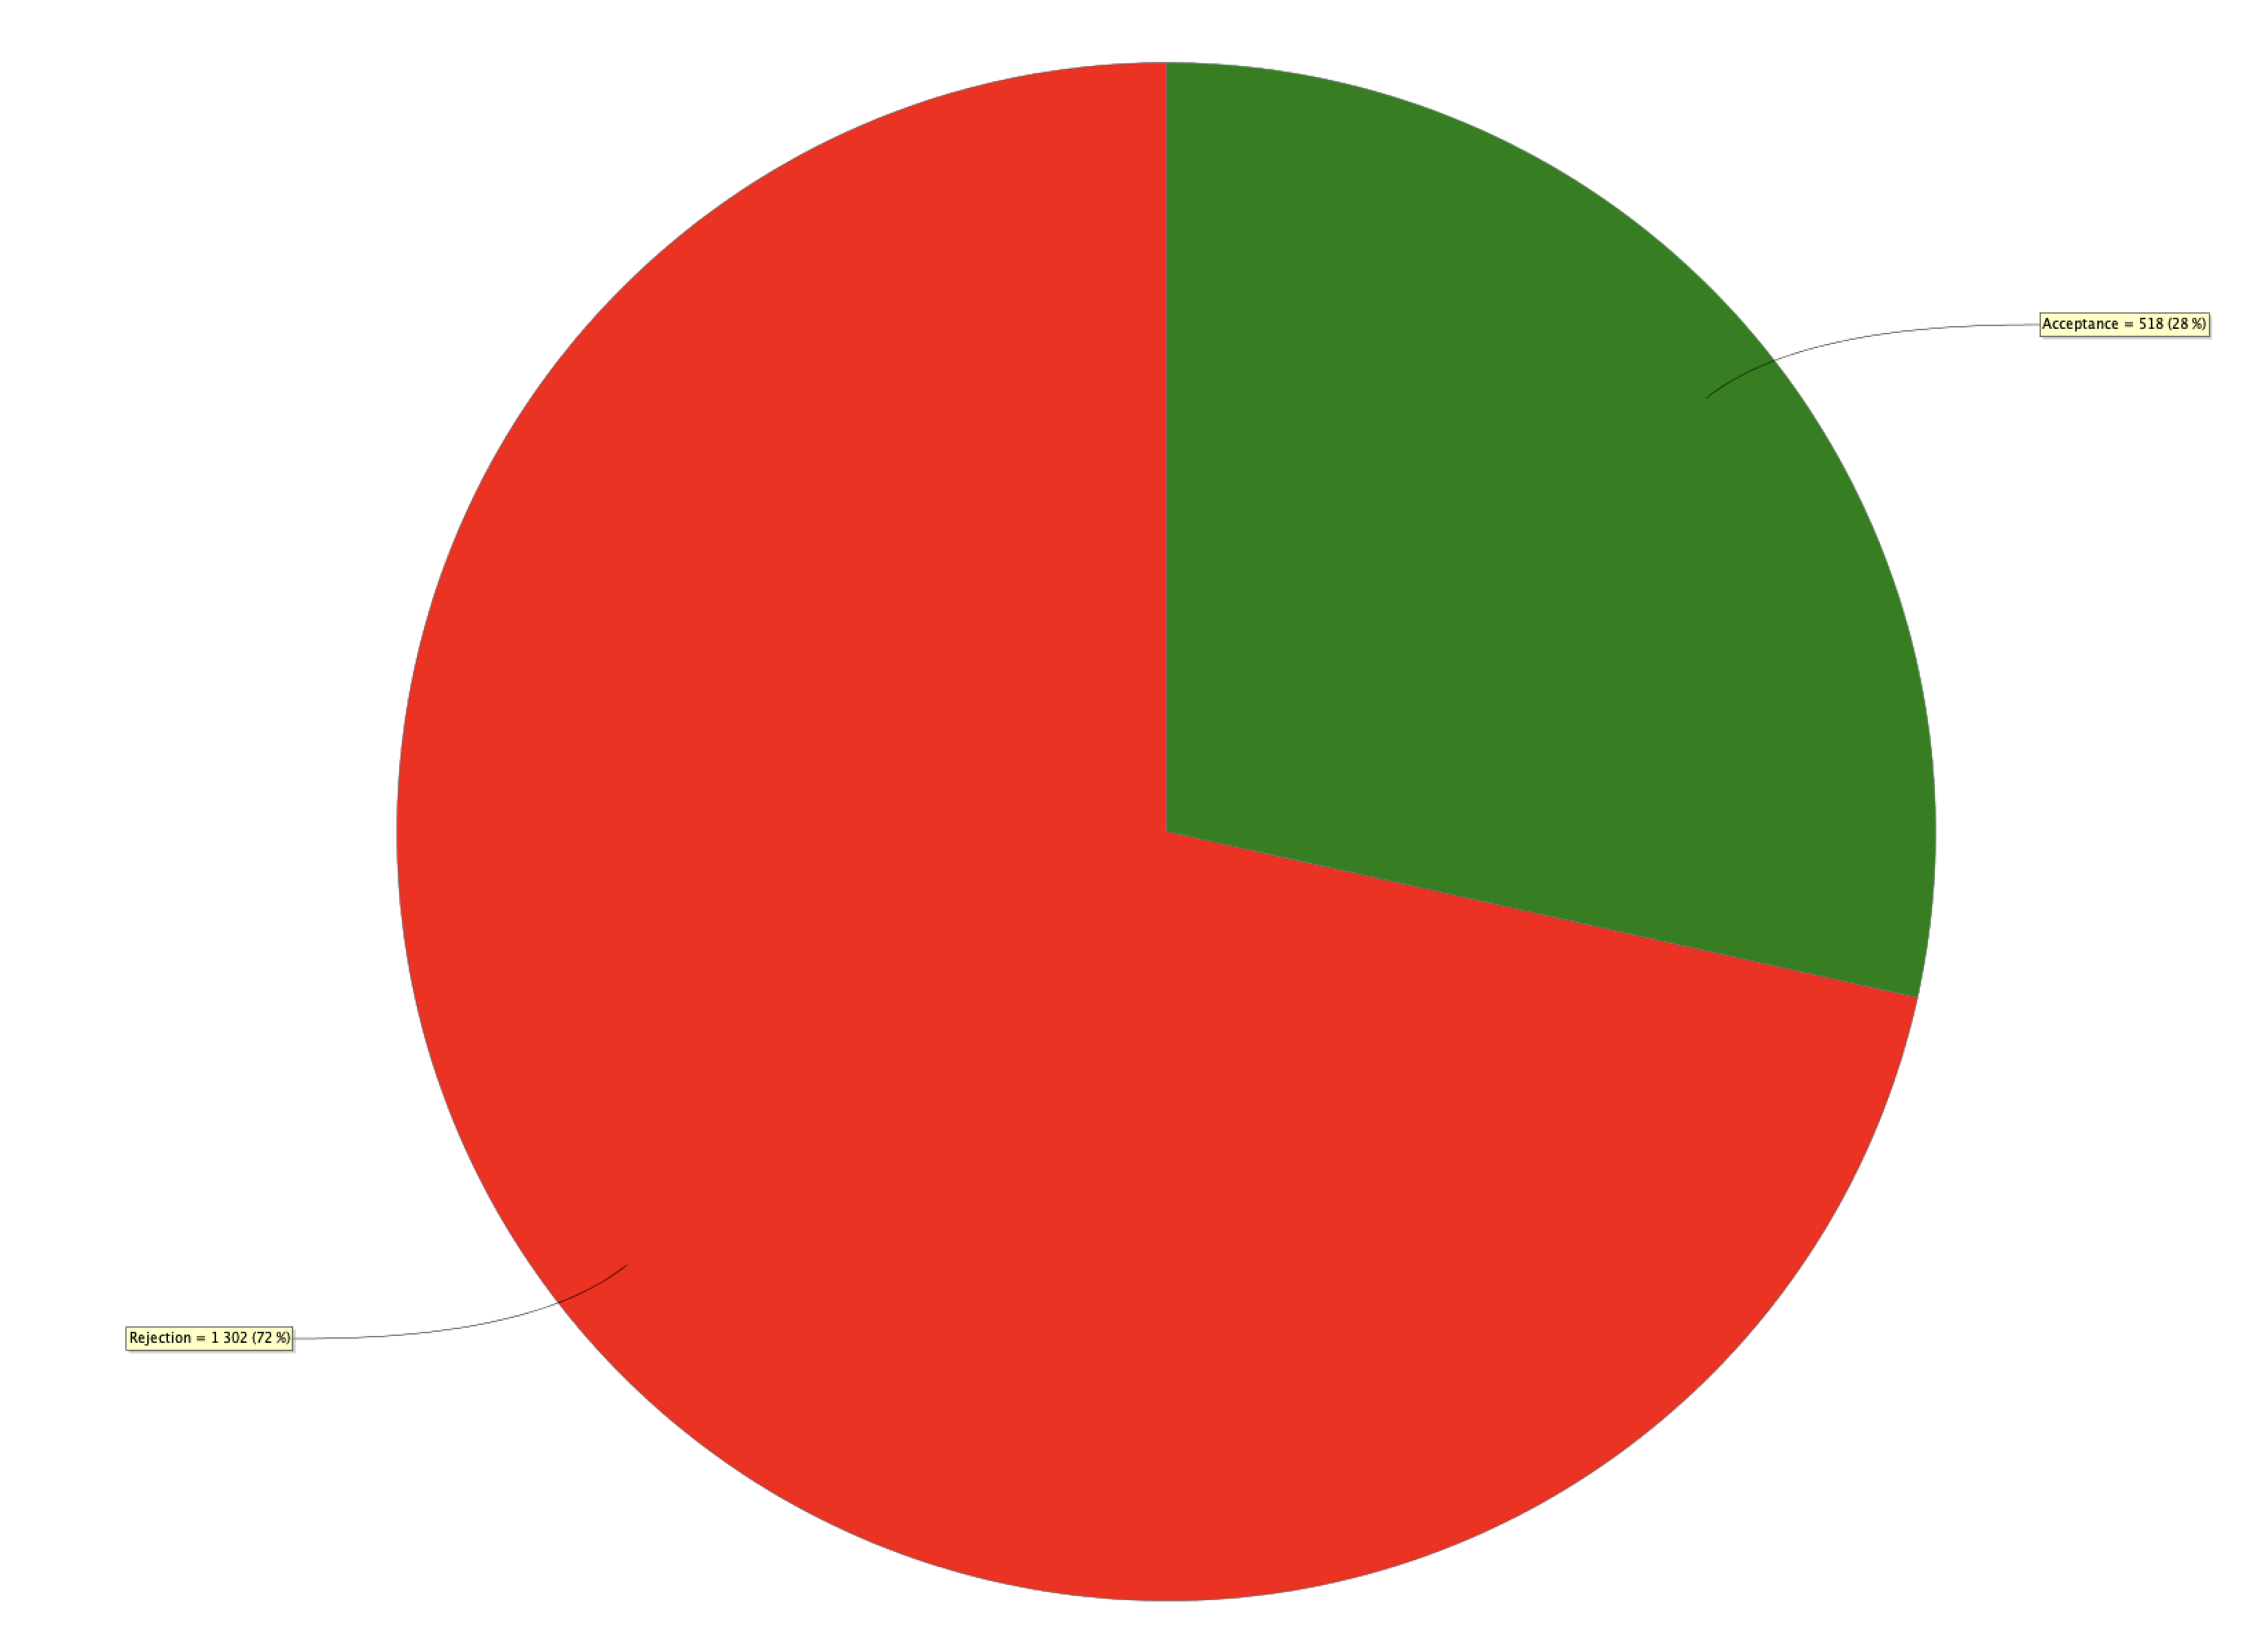
\includegraphics[scale=0.05]{notimelimit.png}\par
\end{center}

\subsubsection{Giving priority to the agent rules attributes}
As described in an earlier sections it was stated that personality trait have absolute priority over the agent rule attributes. By changing the personality traits to 10 which makes the receiving guest always accept the proposal based on personality trait, not including agent rules, the acceptance rate increases to ~71\%.

\begin{center}{}
\centering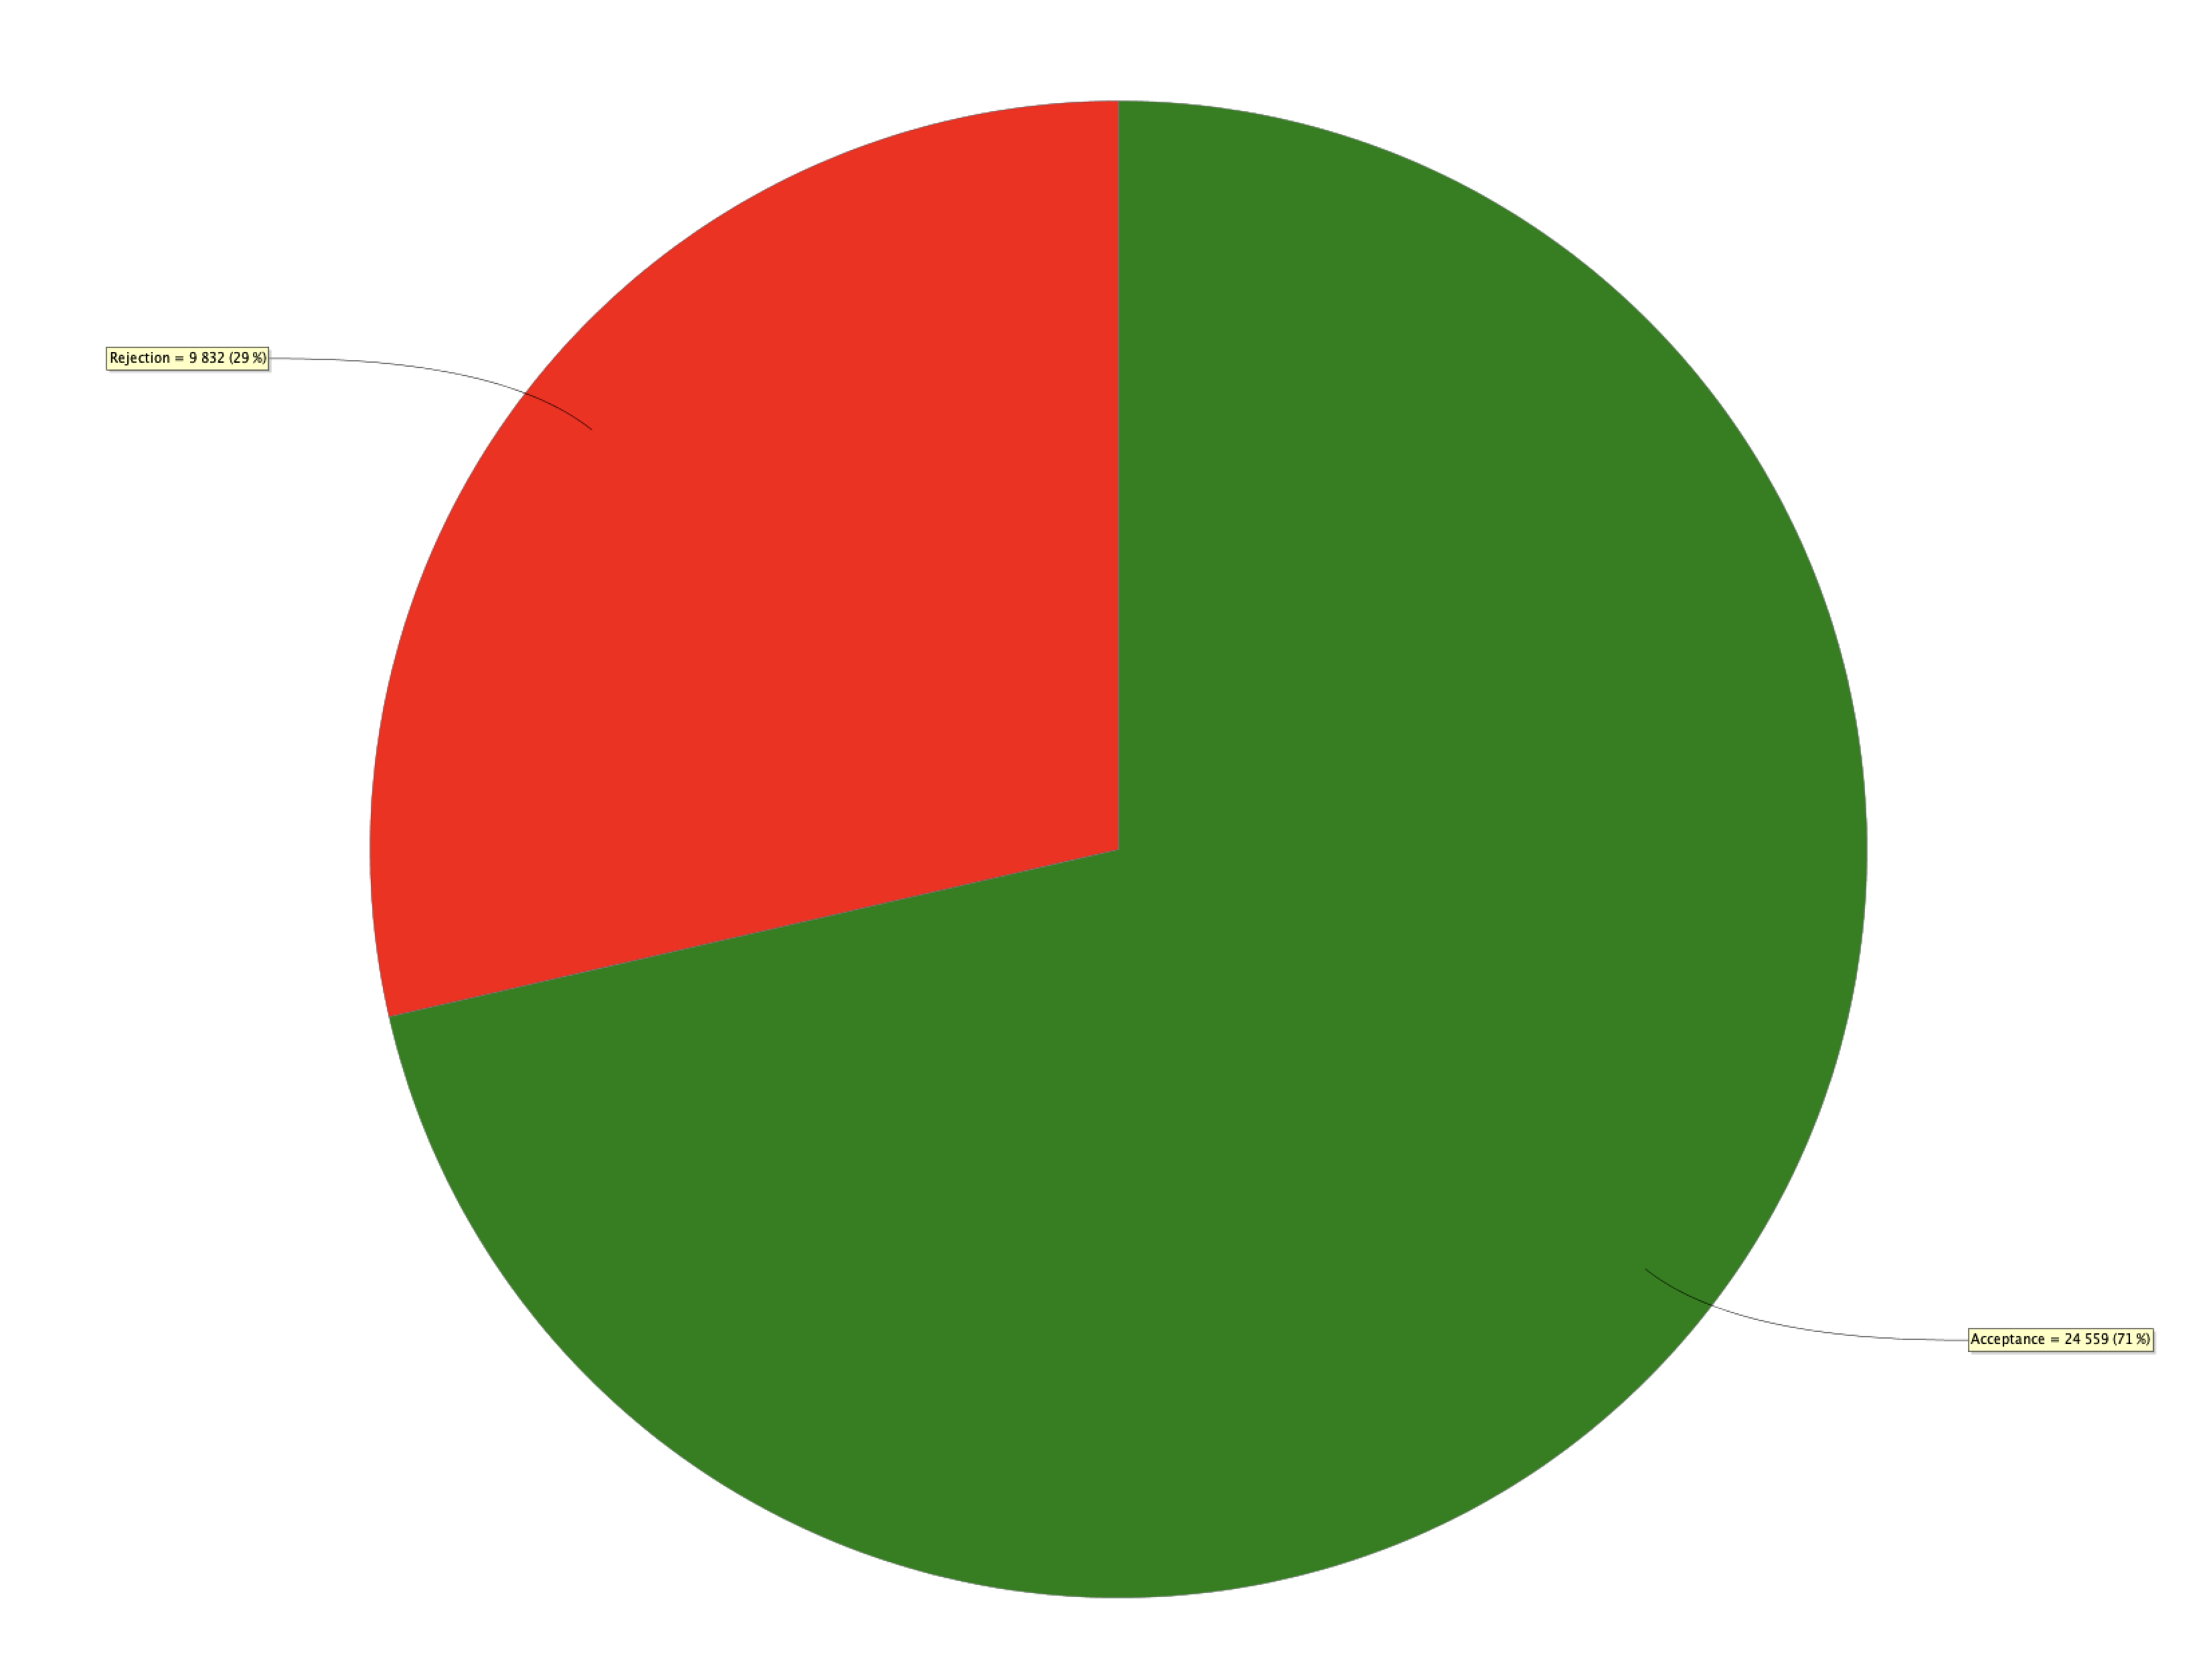
\includegraphics[scale=0.05]{priority.png}\par
\end{center}

\section{Discussion}
The GAMA platform can provide a valuable introduction for those who want to simulate a model with a multi-agent environment. The high-level language and multi-library support enable users to experiment with advanced techniques, such as reinforcement learning, and the intuitive user interface can attract beginners as well. However, the platform has its limitations and other alternatives provide more targeted and modern solutions for specific problems. 
\section{Conclusion}

\end{document}
